%% Submissions for peer-review must enable line-numbering
%% using the lineno option in the \documentclass command.
%%
%% Preprints and camera-ready submissions do not need
%% line numbers, and should have this option removed.
%%
%% Please note that the line numbering option requires
%% version 1.1 or newer of the wlpeerj.cls file, and
%% the corresponding author info requires v1.2

\documentclass[fleqn,10pt,lineno]{wlpeerj} % for journal submissions

% ZNK -- Adding headers for pandoc

\setlength{\emergencystretch}{3em}
\providecommand{\tightlist}{
\setlength{\itemsep}{0pt}\setlength{\parskip}{0pt}}
\usepackage{lipsum}
\usepackage[unicode=true]{hyperref}
\usepackage{longtable}


% Pandoc syntax highlighting
% See https://github.com/rstudio/rticles/issues/182


% Pandoc Header
\usepackage{lipsum}
\usepackage{booktabs}
\usepackage{longtable}
\usepackage{array}
\usepackage{multirow}
\usepackage{wrapfig}
\usepackage{float}
\usepackage{colortbl}
\usepackage{pdflscape}
\usepackage{tabu}
\usepackage{threeparttable}
\usepackage{threeparttablex}
\usepackage[normalem]{ulem}
\usepackage{makecell}
\usepackage{xcolor}

\title{Assesment of the detection distance of an autonomous recording unit in
the cloud forest}

\author[1]{Amauri Sarmiento-Rojas}

\corrauthor[1]{Amauri Sarmiento-Rojas}{\href{mailto:amauri.sarmiento@gmail.com}{\nolinkurl{amauri.sarmiento@gmail.com}}}
\author[1]{Miguel Equihua}

\author[1]{Octavio Pérez-Maqueo}

\author[2]{Brian Napoletano}


\affil[1]{Red de Ambiente y Sustentabilidad, Instituto de Ecología, A.C. Carretera
Antigua a Coatepec 351, El Haya, 91070, Xalapa, Veracruz, Mexico.}
\affil[2]{Centro de Investigaciones en Geografía Ambiental, Universidad Nacional
Autónoma de México. Antigua Carretera a Pátzcuaro 8701, Ex-Hacienda de
San José de la Huerta, 58190, Morelia, Michoacán, Mexico.}


%
% \author[1]{First Author}
% \author[2]{Second Author}
% \affil[1]{Address of first author}
% \affil[2]{Address of second author}
% \corrauthor[1]{First Author}{f.author@email.com}

% 

\begin{abstract}
Passive acoustic monitoring is an efficient and non-intrusive
fundamental tool to provide information on the dynamics of spatial and
temporal activity of the animals that produce sound, which is one of the
research purposes in the emerging field of Ecoacoustics. For designing
studies it is relevant to know the device detection space. The
evaluation of this range distance is a rather complex task, given that
in the sound transmission there are multiple factors related to:
acoustic attributes of the signal of interest, characteristics and
configuration of the recording equipment, as well as some elements of
the habitat and the environment (humidity, temperature, wind,
precipitation, vegetation, topography, etc.). In the present project,
using an experimental approach, we evaluated the range of scope of the
omnidirectional microphone integrated in an automated recorder.
Particularly, we identified the maximum distance at which the animals'
sounds, contrasting in frequency and call structure, are captured.
Additionally, we analysed the effect of distance, terrain slope, tree
density and canopy cover on the loss of signals.
% Dummy abstract text. Dummy abstract text. Dummy abstract text. Dummy abstract text. Dummy abstract text. Dummy abstract text. Dummy abstract text. Dummy abstract text. Dummy abstract text. Dummy abstract text. Dummy abstract text.
\end{abstract}

\begin{document}

\flushbottom
\maketitle
\thispagestyle{empty}

\hypertarget{introduction}{%
\section*{Introduction}\label{introduction}}
\addcontentsline{toc}{section}{Introduction}

Human alteration of ecosystems is affecting severely the diversity of
life on Earth, being the land-use change and climate change the two
major threats on terrestrial ecosystems(Sala et al. 2000; Primack 2010).
Acoustic monitoring offers an efficient and effective method to assess
biodiversity (Riede 1993). Automated Recording Digital Systems (ADRS)
constitute the fundamental equipment to record the sound environment at
a specific site (Acevedo and Villanueva-Rivera 2006). Although there is
a variety of acoustic sensors, it is necessary to improve the technique
to achieve greater representation of biodiversity and to know the
resolution of the study, useful to predict and spatialize the patterns
of acoustic activity. The probability of detecting an animal typically
depends on its distance to the observer or the sensor (Marques et al.
2013). However, few studies have mentioned the maximum range or the area
covered by the recording devices (Llusia, Márquez, and Bowker 2012). It
is relevant to consider that the reaching distance of the devices
delimits the \emph{detection space} of the soundscape or the acoustic
community of interest. Sound energy, measured in decibels (dB) as
amplitude and that is commonly understood as sound intensity, decreases
or attenuates when sound waves propagate in the medium. The sound
attenuation phenomenon is due to three main factors: distance spreading,
absorption of the medium (heat conduction, viscosity or losses due to
molecular relaxation), and other phenomena of wave dispersion
(reflection, refraction, diffraction, and absorption by changes in the
impedance of the medium) (Sueur 2018). The absorption of the medium and
the dispersion phenomena are difficult to model since they depend on
several parameters such as frequency, humidity, temperature, pressure
and physical properties of the obstacles that generate dispersion; on
the contrary, spreading losses are easier to predict if there is a
\emph{reference intensity} and a \emph{reference distance} (Sueur 2018).

The amplitude of the signal at the source (\emph{source level}) can be
extremely different between species and cause marked differences in
detection distances (Llusia, Márquez, and Bowker 2012). In addition, the
sound loses power according to its frequency (measured in Hz);
high-pitched tones (higher frequency) fade faster with distance, because
these signals contains less pressure or energy and easily degrade with
obstacles; in contrast, low-pitched tones (lower frequency) can travel
longer (Marten, Quine, and Marler 1977; Sueur 2018). The structure and
density of vegetation, topography and climatic variables (such as
precipitation, wind speed, air temperature and ambient humidity), are
some of the attributes of the site that can affect the transmission of
sounds in the environment (Aylor 1972; Marten, Quine, and Marler 1977).
On the other hand, among the characteristics of the microphone of the
recorder that can intervene in the reception of the signal of interest
are: the height above ground level, the orientation and/or the detection
angle, as well as the microphone gain or level of recording.

Therefore, the evaluation of the recording range is a fairly complex
task, since many factors are involved in the transmission of the sounds,
from the acoustic nature of the signal of interest and the geophysical
attributes of the site to the characteristics and configuration of the
recording equipment. This study has applications in the field of
Ecoacoustics research, which studies the ecological relevance of
wildlife sounds.

In this project, we evaluated through an experimental approach, the
detection range of the omnidirectional microphone integrated into the
automatic recorder \emph{SWIFT}.

In particular, we aimed: - to identify the maximum distance at which all
the sounds of animals of different frequencies are captured, - to
compare the attenuation of each tested signal according to its frequency
category and its expected attenuation, and - to analyze the effect of
the distance, the terrain slope, the canopy cover and the density of
arboreal vegetation on the loss of the signals.

Since the intensity of the sounds decreases with distance and this
attenuation is favored in the presence of barriers such as vegetation,
we expected a greater loss of amplitude occurring in closer distances
and in sites with higher canopy coverage and tree density. On the other
hand, given the inverse relationship between the distance and the
frequency of the signal, we expect that the sounds with high dominant
frequency will be attenuated in closer distances.

\hypertarget{methods}{%
\section*{Methods}\label{methods}}
\addcontentsline{toc}{section}{Methods}

\hypertarget{experimental-design}{%
\subsection*{Experimental design}\label{experimental-design}}
\addcontentsline{toc}{subsection}{Experimental design}

\paragraph{Study area.}

The experiment was conducted in the Francisco Javier Clavijero Natural
Protected Area, which presents secondary vegetation of the cloud forest,
located in the southwest of the city of Xalapa, Veracruz. We chose six
transects contrasting in tree density, physiographic form, and terrain
slope; one of these (transect 6) can approach a control site because of
the flat terrain (less than 10 of inclination) and low tree density,
located in the Clavijero Botanical Garden. The fieldwork was carried out
on May 8, 2018, from 11:00 a.m. to 5:00 p.m.; this schedule with the
purpose of avoiding the peaks of activity of the local fauna that as
background noise could cause masking of the signal of interest. During
this period, the weather was with was abundant cloudiness, without
precipitation, and no gusts of wind. The air temperature varied between
19.7 and 22.2 C, while the relative humidity changed between 92.3 and
99.9\%; These variables were recorded with a portable meteorological
Microstation \emph{Kestrell 4500}.

\paragraph{Characterization of site.}

We estimated the tree density along each the transect, a circular plot
of 5m radius was drawn at each test point and within this area (78.5
m\^{}2) we counted the number of trees with DAP\textgreater{} 10cm. We
also shot photographs to estimate the percentage of canopy coverage
using the \emph{ImageJ} program. Finally, we calculated the average
slope of the terrain using a laser hypsometer \emph{Nikon Forestry Pro}.
This topographic variable was recorded pointing at a distance of 15m
from the speaker's point to the four cardinal points. This process was
repeated in the six points of each transect (Figure
\ref{fig:studyarea}).

\begin{figure}

{\centering 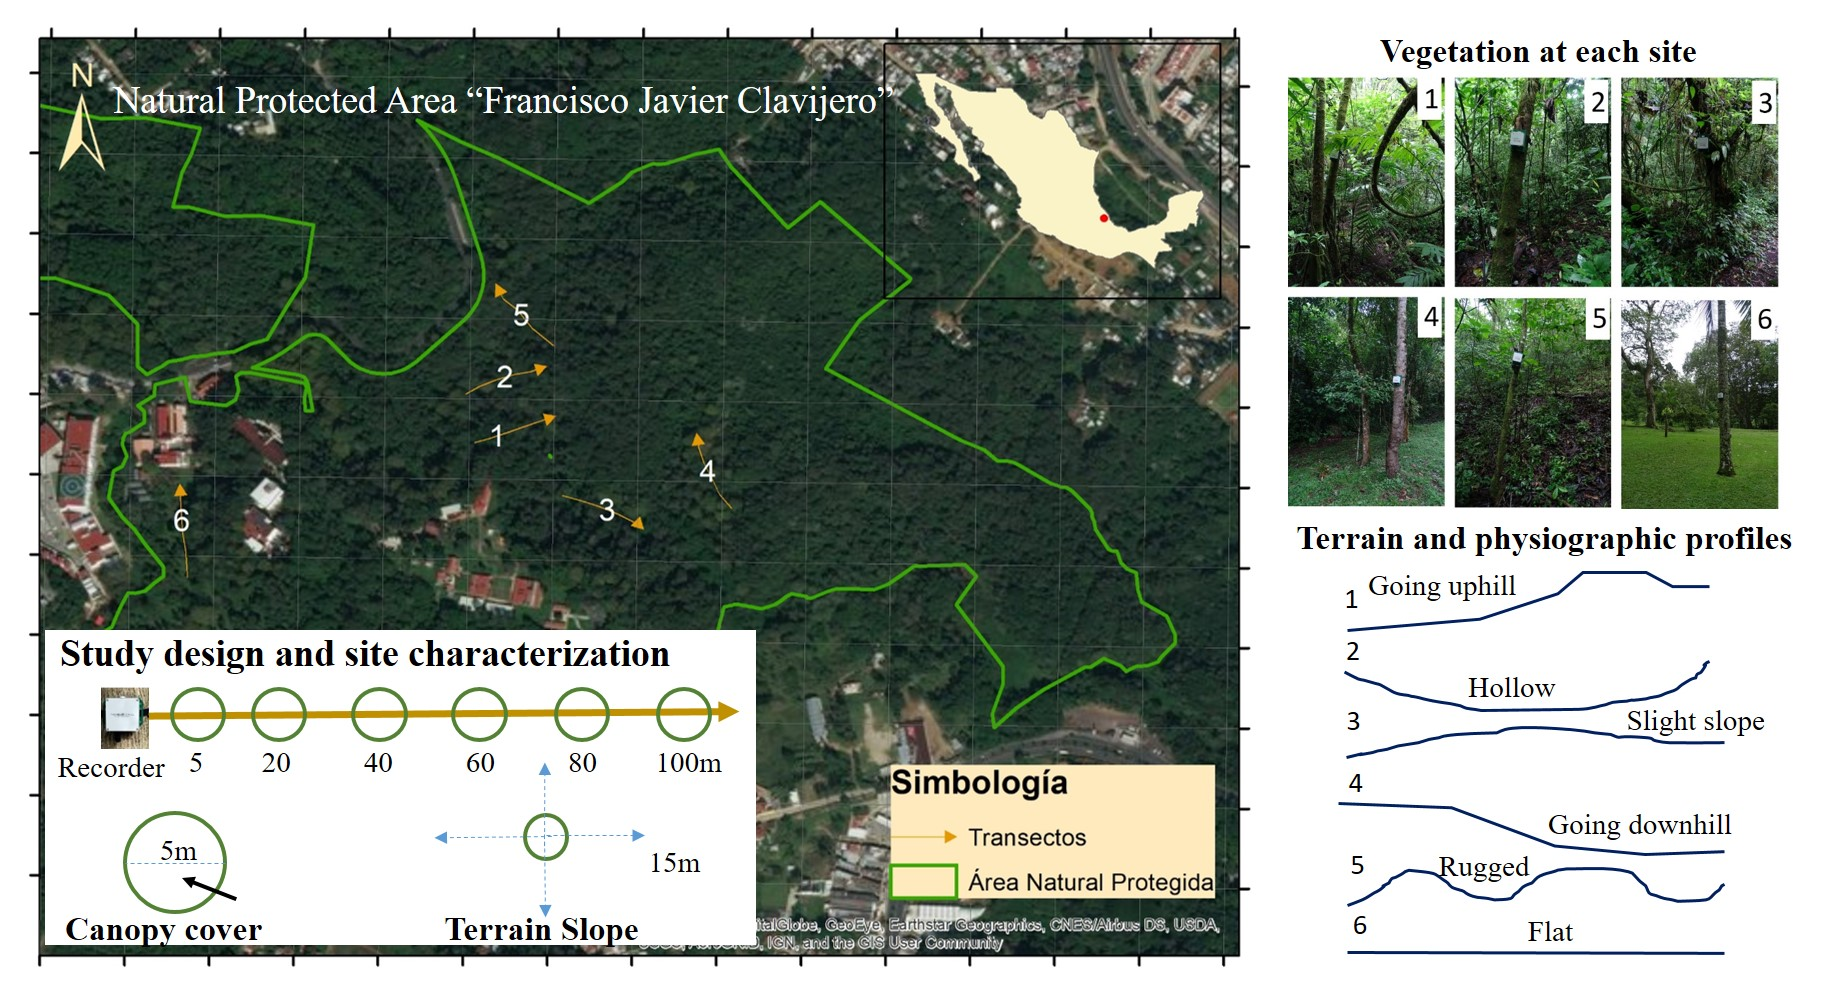
\includegraphics[width=1\linewidth]{RD_studyarea} 

}

\caption{Study area and experimental design indicating the location of the six transects, some representative photographs of the vegetation, as well as the physiographic forms according to each terrain profile.\label{fig:studyarea}}\label{fig:studyarea}
\end{figure}

\paragraph{Recording settings.}

We evaluated the automatic recorder \emph{SWIFT} which comes with a PUI
Audio integrated microphone with an omnidirectional polar pattern (360
as detection angle) and a frequency response of 50 Hz to 16 kHz
(TheCornellLab 2018). We configured the device to record audio
continuously, at a recording rate of 48 kHz and with a microphone gain
set at 35 \emph{dB} (default value). We carried an experiment to know
the maximum recording distance (m), this consisted of reproducing a and
re-recording a soundtrack containing prerecorded animals contrasting in
their dominant frequency (that one with the highest energy). The
detection space was considered as the reach distance from the signal
source, in which its amplitude remains above a minimum detection
threshold (Brenowitz 1982).

\hypertarget{animal-sounds-used-for-tests}{%
\subsection*{Animal sounds used for
tests}\label{animal-sounds-used-for-tests}}
\addcontentsline{toc}{subsection}{Animal sounds used for tests}

We chose representatives of different taxonomic groups with
vocalizations in different categories of dominant frequency: low,
\textless2000 Hz; medium, \textgreater2000 and \textless3000 Hz; and
high, \textgreater{} 3000 Hz. The chosen sounds belong to ten species of
vertebrate animals (three amphibians, one reptile, five birds and one
mammal) (Figure \ref{fig:spectrogram}). These audios were reproduced in
each transect at six distances (5, 20, 40, 60, 80 and 100 m) from the
evaluated microphone. In the original audios, we measured its dominant
frequency (Hz) and its reference amplitude (\emph{iref}), measured in dB
at a reference distance of 1m (\emph{dref}); these were the base
parameters to compare with the outputs from the analysis of the audios
rewritten by the \emph{SWIFT} device. In addition, to take into account
the spectral complexity of the sound, we estimated the acoustic
diversity index (ADI), which measures the signal entropy by measuring
the acoustic activity occurring in 500-Hz frequency bands
(Villanueva-Rivera et al. 2011). This variable was calculated using
``soundecology'', an R library designed for acoustic analysis
(Villanueva-Rivera and Pijanowski 2015) (Table\ref{tab:sounds10spp}).

\begin{figure}

{\centering 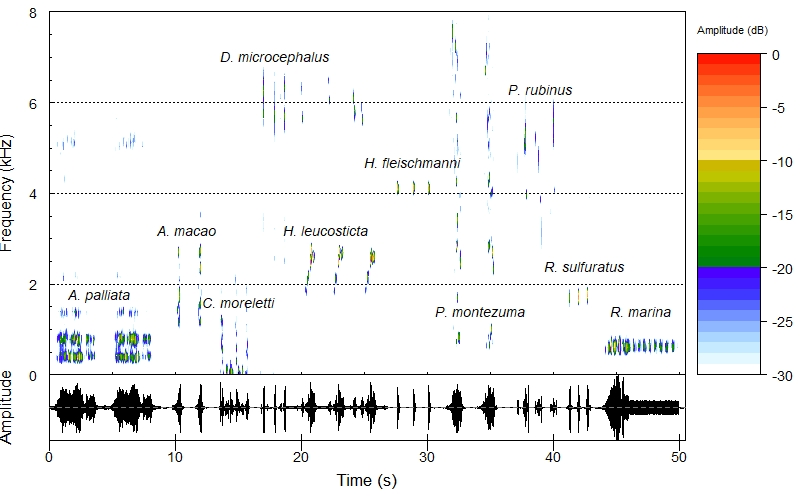
\includegraphics[width=1\linewidth]{espectrog} 

}

\caption{Spectrogram of the selected audios for the experiment, belonging to the ten species of vertebrate animals.\label{fig:spectrogram}}\label{fig:spectrogram}
\end{figure}

\begin{landscape}\begin{table}

\caption{\label{tab:sounds10spp}Description of animal sounds used for tests.\label{tab:sounds10spp}}
\centering
\resizebox{\linewidth}{!}{
\fontsize{8}{10}\selectfont
\begin{tabular}[t]{c|>{}ll>{\em}llcrr>{\bfseries}rcc}
\toprule
Sp. & Group & Common name & Scientific name & Sound content & Author of recording & Duration (s) & Amplitude (dB) & Frecuencia (Hz) & Frequency category & ADI value\\
\midrule
1 & Reptiles & Morelet's Crocodile & Crocodylus morelletti & 3 calls & SKPC & 2.5 & -28.0 & 387 & low & 4.76\\
2 & Amphibians & Cane Toad & Rhinella marina & 1 trill & ASR & 9.0 & -3.5 & 657 & low & 4.85\\
3 & Mammals & Mantled Howler Monkey & Allouata palliata & 2 calls & ASR & 10.0 & -16.8 & 779 & low & 4.97\\
4 & Birds & Keel-billed Toucan & Ramphastos sulfuratus & 3 songs & ASR & 2.0 & -16.1 & 1721 & low & 4.66\\
5 & Birds & White-breasted Wood-wren & Henicorhina leucosticta & 3 songs & FGG & 8.0 & -22.6 & 2507 & medium & 4.03\\
6 & Birds & Scarlet Macaw & Ara macao & 2 calls & ASR & 5.0 & -24.6 & 2701 & medium & 2.93\\
7 & Birds & Montezuma Oropendola & Psarocolius montezuma & 2 songs & ASR & 8.0 & -22.5 & 2809 & medium & 4.97\\
8 & Amphibians & Fleischmann's Glass Frog & Hyalinobatrachium fleischmanni & 3 calls & ASR & 3.0 & -21.4 & 4062 & high & 4.92\\
9 & Birds & Common Vermilion Flycatcher & Pyrocephalus rubinus & 3 songs & ASR & 3.5 & -36.4 & 5057 & high & 4.31\\
10 & Amphibians & Small-headed Treefrog & Dendropsophus microcephalus & 3 calls & ASR & 2.0 & -30.3 & 6231 & high & 2.67\\
\bottomrule
\end{tabular}}
\end{table}
\end{landscape}

To standardize the intensity of the sounds, these were normalized to -4
dB using the free-use software \emph{Audacity}. The recorder
\emph{SWIFT} was placed at a height of 2m above ground level. To play
the audios we used a portable loudspeaker \emph{XP8000RD Power\&Co} that
has a power of 4200 W. The volume was calibrated at an average intensity
of 55 dB measured at 1m distance, as reference distance (\emph{dref}),
and at a height of 1m above the ground.

\hypertarget{assessment-of-the-detection-space}{%
\subsection*{Assessment of the detection
space}\label{assessment-of-the-detection-space}}
\addcontentsline{toc}{subsection}{Assessment of the detection space}

In each recording obtained and for the ten signals of interest, the
spectrum analysis tool
\href{file:///C:/Program\%20Files\%20(x86)/Audacity/help/manual/man/plot_spectrum.html}{\emph{Plot
Spectrum}} was used in the \emph{Audacity} program to measure the
dominant frequency measured in number of cycles per second or Hertz
(Hz), as well as its amplitude in decibels at full scale
(\href{https://en.wikipedia.org/wiki/DBFS}{dBFS}).

Let \(X_{11}, X_{12},\ldots X_{ij}\) be the measures of observed
amplitude in the tested distances (\(i = 6\)) and sites (\(j = 6\)), for
each signal of interest (or species). We averaged these amplitude values
taking into account the logarithmic nature of this variable, using the
formula: \[Amplitude_{obs} = \frac{10^{Amplitude_{dB}*{-1}}}{10}\]

After transformed, these values were added and divided by the number of
observations (\(n = 36\)) and again transformed back into digital
amplitude (dBFS).

\[Amplitude_{obs(mean)} = \frac{X_{obs1} + X_{obs_2} + \cdots + X_{obsn}} {n}
      = \frac{1}{n}\sum_{i}^{n} Amplitude_{i} \]

From the reference amplitude value, the acoustic extinction curves were
constructed for each distance. The detection threshold occurs when a
loss of the signal of interest is identified; that is, when it is no
longer displayed on the spectrogram; in this case, we assigned a
symbolic value of -100 dBFS.

\hypertarget{attenuation-analysis-by-animal-sound-type}{%
\subsection*{Attenuation analysis by animal sound
type}\label{attenuation-analysis-by-animal-sound-type}}
\addcontentsline{toc}{subsection}{Attenuation analysis by animal sound
type}

To study the observed attenuation with respect to distance for each
species, and according to its dominant frequency category; the expected
attenuation curve was generated according to the theory of sound
propagation. The following formula was used to calculate these values:
\(Amplitud_{expected} = I_{ref}-20*log(d/d_{ref})\); where the expected
amplitude \((Amplitude_{expected})\) is obtained from the reference
amplitude \((I_{ref})\), the distance of interest \((d)\) and the
reference distance \((d_{ref})\).
\href{https://www.omnicalculator.com/physics/distance-attenuation\#inverse-square-law}{Distance
attenuation calculator}

\hypertarget{effects-of-topography-and-vegetation}{%
\subsection*{Effects of topography and
vegetation}\label{effects-of-topography-and-vegetation}}
\addcontentsline{toc}{subsection}{Effects of topography and vegetation}

To study the possible effect of topography and vegetation on signal
reception, for each species, we made linear models of the measurements
of amplitude observed in full scale (dBFS) in function of the expected
amplitude (dbFS), the recording distance (m), the average slope of the
site, the density of tree stems with DAP\textgreater{} 10cm and the tree
cover percentage. We used the \texttt{glmulti} function to find the most
appropriate model based on the \emph{corrected Akaike Information
Criteria (AICc)}.

\hypertarget{results}{%
\section*{Results}\label{results}}
\addcontentsline{toc}{section}{Results}

\hypertarget{detection-space-of-tested-recorder}{%
\subsection*{Detection space of tested
recorder}\label{detection-space-of-tested-recorder}}
\addcontentsline{toc}{subsection}{Detection space of tested recorder}

We present the acoustic extinction curves generated for each site
(Figure\ref{fig:attenbysite}) and for each species
(Figure\ref{fig:attenbyspp}) based on their average amplitude values, in
decibels at full scale (dBFS), recorded for each distance.

\begin{figure}

{\centering 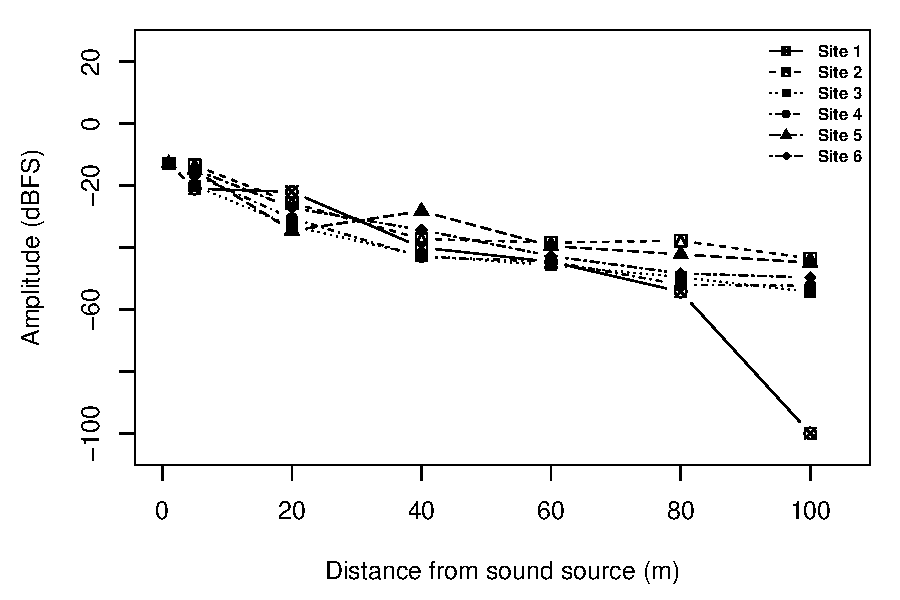
\includegraphics[width=1\linewidth]{ASR_MyPaper_2020_files/figure-latex/attenbysite-1} 

}

\caption{Acoustic extinction curves by site with amplitude measured at six distances.\label{fig:attenbysite}}\label{fig:attenbysite}
\end{figure}

\begin{figure}[H]

{\centering 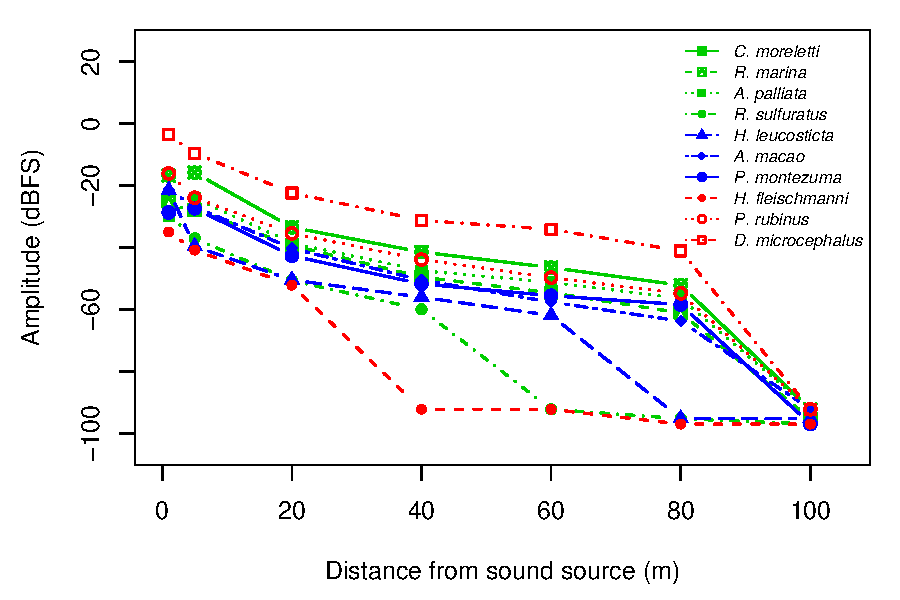
\includegraphics[width=1\linewidth]{ASR_MyPaper_2020_files/figure-latex/attenbyspp-1} 

}

\caption{Acoustic extinction curves by sound type, with amplitude evaluated at six distances. Colors indicate the corresponding peak frequency category that each animal sound: red (high-pitched), blue (medium), green (low-pitched).\label{fig:attenbyspp}}\label{fig:attenbyspp}
\end{figure}

\begin{figure}

{\centering 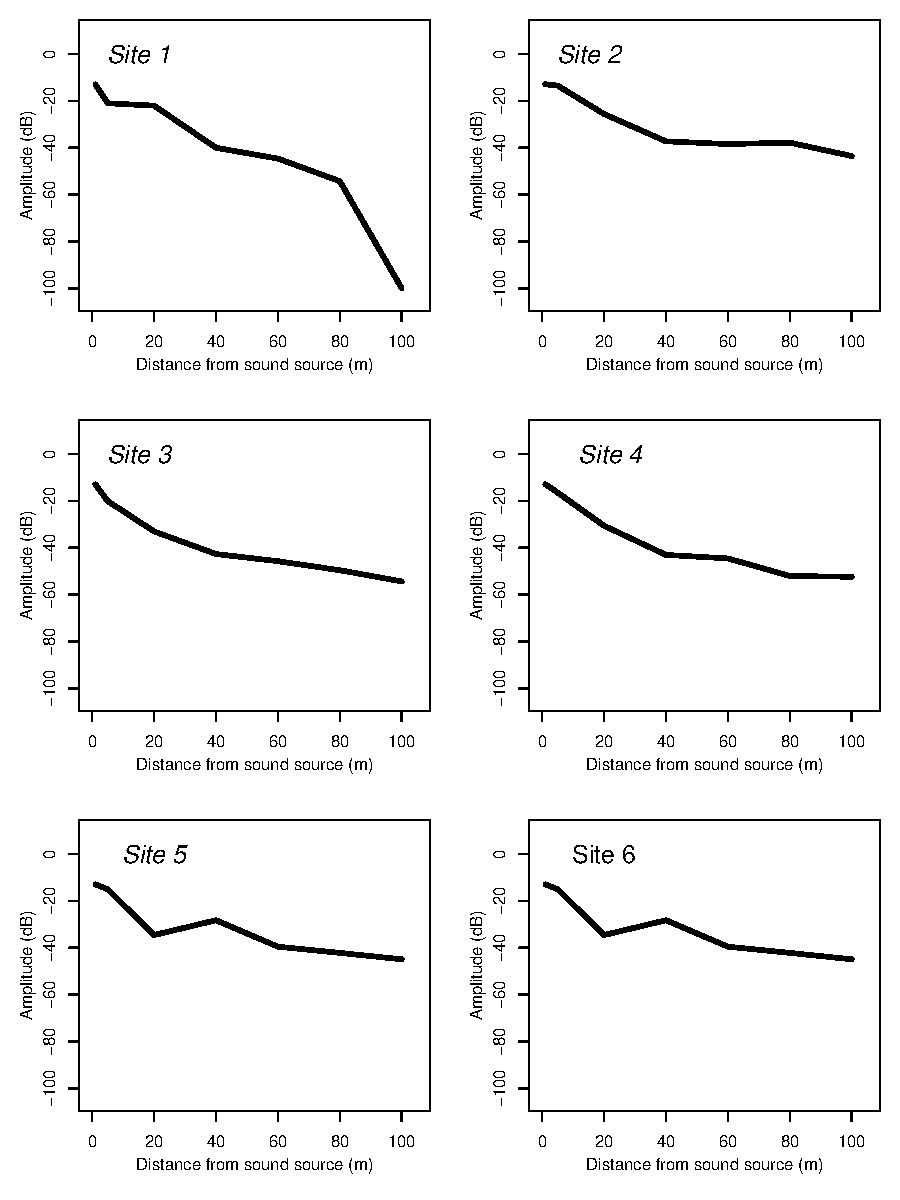
\includegraphics[width=1\linewidth]{ASR_MyPaper_2020_files/figure-latex/curvesxsite-1} 

}

\caption{Attenuation curves with amplitude evaluated at six distances for six sites.\label{fig:curvesxsite}}\label{fig:curvesxsite}
\end{figure}

\hypertarget{atenuattion-by-animal-sound-type}{%
\subsection*{Atenuattion by animal sound
type}\label{atenuattion-by-animal-sound-type}}
\addcontentsline{toc}{subsection}{Atenuattion by animal sound type}

The loss of signal by sound type or species depending on the expected
attenuation was very variable among the different types of sounds. In
most species, the attenuation observed was greater than the expected
curve in the distances closest to the sound source
(Figure\ref{fig:curvesxspp}).

\begin{figure}

{\centering 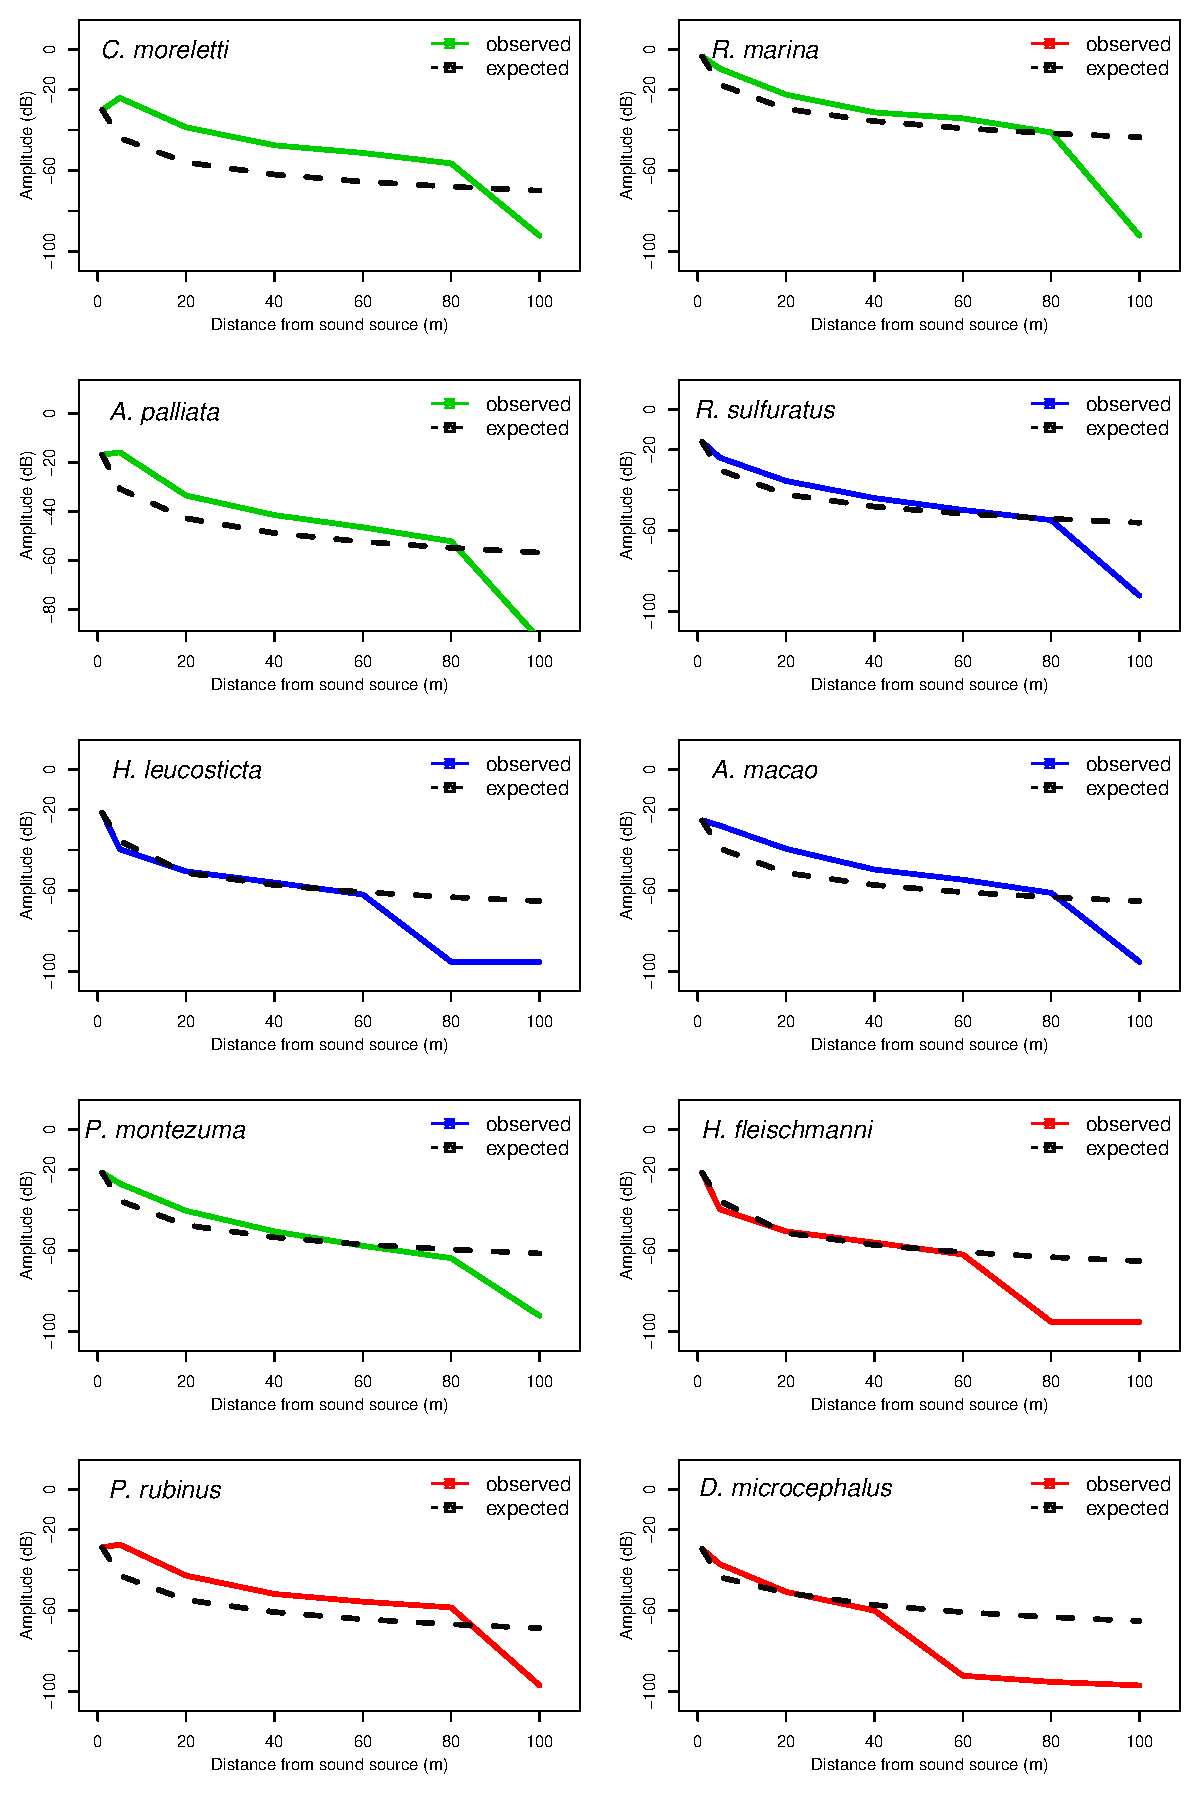
\includegraphics[width=1\linewidth]{ASR_MyPaper_2020_files/figure-latex/curvesxspp-1} 

}

\caption{Observed vs expected attenuation curves of the ten animal sounds, with amplitude measured at six distances. Colors indicate the corresponding category of peak frequency: green for low-, blue for medium- and red for high-pitched sounds.\label{fig:curvesxspp}}\label{fig:curvesxspp}
\end{figure}

\hypertarget{effects-of-topography-and-vegetation-1}{%
\subsection*{Effects of topography and
vegetation}\label{effects-of-topography-and-vegetation-1}}
\addcontentsline{toc}{subsection}{Effects of topography and vegetation}

We studied the detection distance of the recorder in 36 locations (6 by
site) which are contrasting in tree density, canopy cover and terrain
slope (Figure\ref{fig:PCAplot}).

\begin{figure}

{\centering 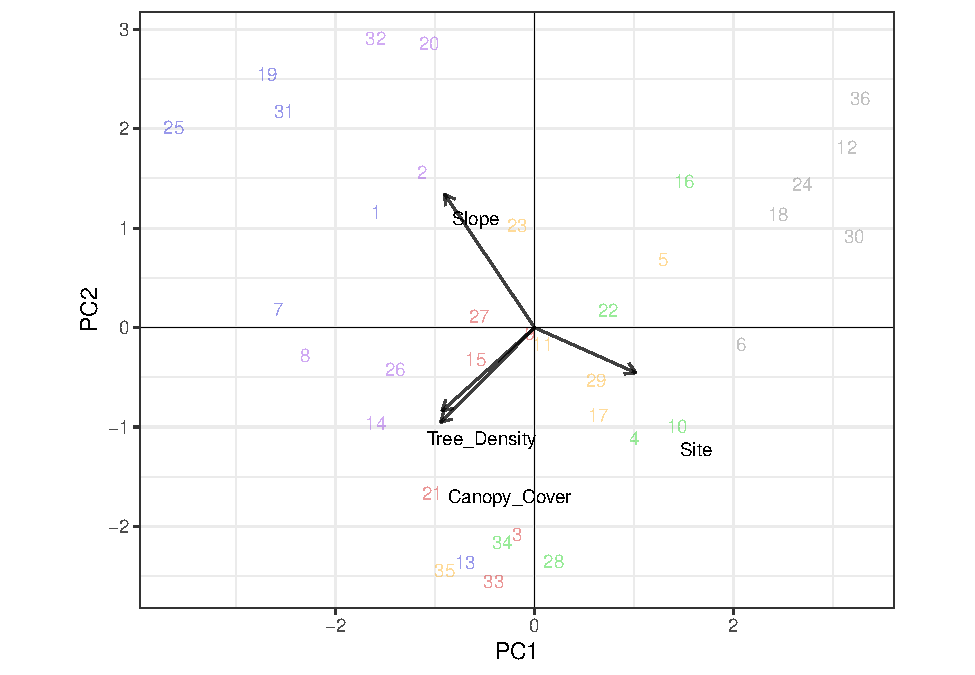
\includegraphics[width=1\linewidth]{ASR_MyPaper_2020_files/figure-latex/PCAplot-1} 

}

\caption{PCA.\label{fig:PCAplot}}\label{fig:PCAplot}
\end{figure}

\hypertarget{linear-model}{%
\subsubsection*{Linear Model}\label{linear-model}}
\addcontentsline{toc}{subsubsection}{Linear Model}

For each one of the species, we present the linear models that were
selected using the ``glmulti'' function (Table\ref{tab:BestModels}).

\begin{landscape}\begin{table}

\caption{\label{tab:BestModels}Linear model results}
\centering
\resizebox{\linewidth}{!}{
\fontsize{8}{10}\selectfont
\begin{tabular}[t]{r>{\em}lrrlrr}
\toprule
Sp. & Common name & Frequency (Hz) & $r^{2}$ & Model & $\alpha$ & $\sigma_{\alpha}$\\
\midrule
1 & Morelet's Crocodile & 387 & 0.671 & $\alpha + Distance$ & -18.072 & 3.054\\
2 & Cane Toad & 657 & 0.710 & $\alpha + Distance + Tree_{Density}:Distance$ & -28.141 & 2.936\\
3 & Mantled Howler Monkey & 779 & 0.690 & $\alpha + Distance$ & -26.021 & 2.662\\
4 & Keel-billed Toucan & 1721 & 0.793 & $\alpha + Distance + Canopy_{Cover}:Distance + Slope:Tree_{Density}$ & -32.339 & 3.288\\
5 & White-breasted Wood-wren & 2507 & 0.750 & $\alpha + Distance + Tree_{Density}:Distance$ & -37.984 & 2.899\\
6 & Scarlet Macaw & 2701 & 0.804 & $\alpha + Distance + Slope:Canopy_{Cover}$ & -25.266 & 2.562\\
7 & Montezuma Oropendola & 2809 & 0.724 & $\alpha + Distance + Canopy_{Cover}:Distance$ & -27.746 & 3.096\\
8 & Fleischmann's Glass Frog & 4062 & 0.718 & $\alpha + Distance + Canopy_{Cover}$ & -19.877 & 7.200\\
9 & Common Vermilion Flycatcher & 5057 & 0.740 & $\alpha + Distance + Slope:Distance$ & -23.489 & 2.555\\
10 & Small-headed Treefrog & 6231 & 0.668 & $\alpha + Distance + Slope:Distance + Slope:Canopy_{Cover}$ & -17.170 & 5.262\\
\bottomrule
\end{tabular}}
\end{table}
\end{landscape}

\hypertarget{model-selection-and-fitting-theoretical-vs-empirical-model}{%
\subsection*{Model selection and fitting: theoretical vs empirical
model}\label{model-selection-and-fitting-theoretical-vs-empirical-model}}
\addcontentsline{toc}{subsection}{Model selection and fitting:
theoretical vs empirical model}

The main signal is caught by the intercept, which contains the
\emph{offset} term and it is clearly different from zero. In order to
know the \emph{offtset} effects, we plotted the intercept with its
confidence intervals at 95\%. It is clear that there is a certain common
arrangement for the attenuation of all calls, and the only one that
separates the most is that one with a dominant frequency of 2500 Hz,
which is attenuated apparently more than everyone
(Figure\ref{fig:Intercepts}). In all cases, we found a small effect of
distance with the same sign as the offset, so we could actually add it
to the previous estimate. Then, there are the secondary effects of tree
density, terrain slope and canopy coverage, which as explanatory
variables have small effects compared to the size of the \emph{offset}.

\begin{figure}

{\centering 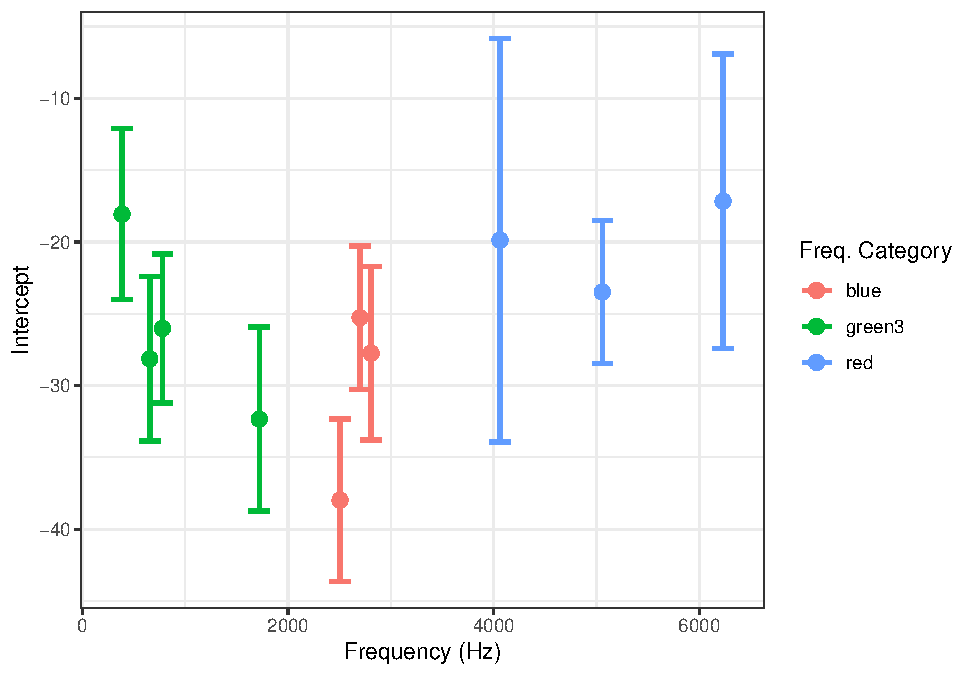
\includegraphics[width=1\linewidth]{ASR_MyPaper_2020_files/figure-latex/Intercepts-1} 

}

\caption{Intercepts showing attenuation by species.\label{fig:Intercepts}}\label{fig:Intercepts}
\end{figure}

\hypertarget{model-contrast-approach}{%
\subsubsection*{Model contrast approach}\label{model-contrast-approach}}
\addcontentsline{toc}{subsubsection}{Model contrast approach}

We proposed a \emph{complete model} as a reference, which contains
theoretical attenuation as a term plus an ``empirical'' component
constructed with the main effects of distance and of site conditions
including its first-order interactions. From this reference model, the
non-significant terms are removed to get a ``minimum adequate model''.
Based on the estimates of the ``additive explanatory'' effect of the
``empirical'' components, we assessed the improvement that the empirical
model can bring to the theoretical model (Table\ref{tab:Modelcontrast}).
We see no significant improvements, except in the case of
\emph{White-breasted Wood-wren}.

\begin{table}[!h]

\caption{\label{tab:Modelcontrast}Contrast of the theoretical vs empirical model}
\centering
\resizebox{\linewidth}{!}{
\fontsize{8}{10}\selectfont
\begin{tabular}[t]{r>{\em}lrcccccc}
\toprule
Sp. & Common name & Frequency (Hz) & Model & $r^{2}_{theoretical}$ & df residual & df model & F & P\\
\midrule
1 & Morelet's Crocodile & 387 & theoretical vs empirical & 0.754 & 27 & 7 & 1.103 & 0.389\\
2 & Cane Toad & 657 & theoretical vs empirical & 0.724 & 27 & 7 & 1.222 & 0.325\\
3 & Mantled Howler Monkey & 779 & theoretical vs empirical & 0.770 & 27 & 7 & 1.187 & 0.343\\
4 & Keel-billed Toucan & 1721 & theoretical vs empirical & 0.810 & 27 & 7 & 2.287 & 0.058\\
5 & White-breasted Wood-wren & 2507 & theoretical vs empirical & 0.787 & 27 & 7 & 5.224 & 0.001\\
6 & Scarlet Macaw & 2701 & theoretical vs empirical & 0.845 & 27 & 7 & 1.814 & 0.125\\
7 & Montezuma Oropendola & 2809 & theoretical vs empirical & 0.734 & 27 & 7 & 1.647 & 0.165\\
8 & Fleischmann's Glass Frog & 4062 & theoretical vs empirical & 0.758 & 27 & 7 & 1.847 & 0.119\\
9 & Common Vermilion Flycatcher & 5057 & theoretical vs empirical & 0.780 & 27 & 7 & 1.772 & 0.134\\
10 & Small-headed Treefrog & 6231 & theoretical vs empirical & 0.710 & 27 & 7 & 1.851 & 0.118\\
\bottomrule
\end{tabular}}
\end{table}

We can also explore the convenience of adding some of the site
characterization variables or an additional distance effect. The
principal effects of these variables plus the term of \emph{theoretical
attenuation}. Using the \emph{stepwise} strategy but without
incorporating any interaction in order to make slight improvements that
may more clearly have the contextual effect of the site's
characteristics on the sound behavior.

\hypertarget{do-all-calls-fade-in-the-same-way-does-the-same-model-apply-to-all}{%
\subsubsection*{Do all calls fade in the same way: does the same model
apply to
all?}\label{do-all-calls-fade-in-the-same-way-does-the-same-model-apply-to-all}}
\addcontentsline{toc}{subsubsection}{Do all calls fade in the same way:
does the same model apply to all?}

We adjusted a model including theoretical attenuation in interaction
with the species and of course, the main effects of both. For
convenience, the type of contrast used in R is \emph{treatment}, which
means that one of the conditions is chosen as a reference and all others
are then expressed as the difference from that reference. Usually, the
first treatment is taken as a reference, but anyone that interests may
be chosen.

Almost all species could be modeled similarly, except for the sound of
species 5 \emph{(Henicorhina leucosticta)}.

This model shows that there is no statistically significant change in
relation to the ``original complete model''. All species behaved
similarly to each other, in terms of attenuation in relation to
distance. The species differ in the initial condition from which the
attenuation process begins.

This simplified model seems to account for the data almost as well as
the "original complete model; so, in spite of everything, in the case
tested we could even simplify the model a little more since several
species seem not to differ either when initial condition: Sp1 == Sp3 ==
Sp7 == Sp10. When making this change, the explanatory capacity of around
0.5\% is lost.

\hypertarget{discussion}{%
\section*{Discussion}\label{discussion}}
\addcontentsline{toc}{section}{Discussion}

The maximum average distance at which most of the animal sounds of
different frequencies are detected is 80 m, some sounds are attenuated
and lost at 40m. As we expected, the high-frequency signals resulted in
a greater loss as the distance increases.

The detection space may vary according to weather conditions such as
temperature, humidity, wind, and precipitation, in the field is not
possible to control these environmental variables.

The evaluated site variables of terrain slope and vegetation had no
significant effect \emph{per se} on attenuation. It would be interesting
to study the effect of other topographic variables such as the terrain
roughness, the orientation and the physiographic form of the site.

In the wildlife, animals emit vocalizations at different heights and
some of them move or change orientation while there are calling.

The main purpose of this project was to estimate the detection distance
of the recorder which is especially relevant for studies in which it is
intended to record the sound remotely and autonomously. On the contrary,
it was not the objective of this project to evaluate the transmission of
sounds, which could require another type of experimental design.

\paragraph{Considerations:}

\dots

\begin{enumerate}
\def\labelenumi{\arabic{enumi}.}
\item
  The issue of ``identifiability of the call'' is pending, in the sense
  how much distortion occurs to degrade the characteristics that allow
  differentiating the animals studied?
\item
  There is no reference control signal (pure tone of 1kHz at 94 dB SPL
  which is the pressure of 1 Pascal), based on this normalization would
  be performed.
\item
  Review the frequency response of the horn, you may amplify certain
  frequencies further.
\item
  Consider the sensitivity of the microphone (frequency response and
  gain).
\end{enumerate}

\hypertarget{acknowledgments}{%
\section*{Acknowledgments}\label{acknowledgments}}
\addcontentsline{toc}{section}{Acknowledgments}

To Esau Toaki Villareal Olvera for orientation on acoustic transmission
issues. To Fernando González García (FGG) and Sofía Karen Pérez Cruz
(SKPC) for contributing with some audio files used in this project.

\hypertarget{references}{%
\section*{References}\label{references}}
\addcontentsline{toc}{section}{References}

\hypertarget{refs}{}
\leavevmode\hypertarget{ref-Acevedo2006}{}%
Acevedo, Miguel A., and Luis J. Villanueva-Rivera. 2006. ``Using
automated digital recording systems as effective tools for the
monitoring of birds and amphibians.'' \emph{Wildlife Society Bulletin}
34 (1): 211--14. \url{https://doi.org/10.2193/0091-7648(2006)34}.

\leavevmode\hypertarget{ref-Aylor1972}{}%
Aylor, Donald. 1972. ``Noise reduction by vegetation and ground.''
\emph{The Journal of the Acoustical Society of America} 51 (2):
197--205. \url{https://doi.org/10.1121/1.1912830}.

\leavevmode\hypertarget{ref-Brenowitz1982}{}%
Brenowitz, Eliot A. 1982. ``The active space of red-winged blackbird
song.'' \emph{Journal of Comparative Physiology A} 147 (4): 511--22.
\url{https://doi.org/10.1007/BF00612017}.

\leavevmode\hypertarget{ref-Llusia2012}{}%
Llusia, Diego, Rafael Márquez, and Richard Bowker. 2012. ``Terrestrial
sound monitoring systems, a methodology for quantitative calibration.''
\emph{Bioacoustics: The International Journal of Animal Sound and Its
Recording} 20 (3): 277--86.
\url{https://doi.org/10.1080/09524622.2011.9753651}.

\leavevmode\hypertarget{ref-Marques2013}{}%
Marques, Tiago A., Len Thomas, Stephen W. Martin, David K. Mellinger,
Jessica A. Ward, David J. Moretti, Danielle Harris, and Peter L. Tyack.
2013. ``Estimating animal population density using passive acoustics.''
\emph{Biological Reviews} 88 (2): 287--309.
\url{https://doi.org/10.1111/brv.12001}.

\leavevmode\hypertarget{ref-Marten1977}{}%
Marten, Ken, Douglas Quine, and Peter Marler. 1977. ``Sound transmission
and its significance for animal vocalization: II. Tropical forest
habitats.'' \emph{Behavioral Ecology and Sociobiology} 2 (3): 291--302.

\leavevmode\hypertarget{ref-Primack2010}{}%
Primack, R. B. 2010. \emph{Essentials of conservation biology}.
Sunderland, Massachusetts: Sinaeur Associates.

\leavevmode\hypertarget{ref-Riede1993}{}%
Riede, Klaus. 1993. ``Monitoring Biodiversity: Analysis of Amazonian
Rainforest Sounds.'' \emph{Ambio} 22 (8): 546--48.

\leavevmode\hypertarget{ref-Salaetal2000}{}%
Sala, Osvaldo E., F. Stuart Chapin, Juan J. Armesto, Eric Berlow, Janine
Bloomfield, Rodolfo Dirzo, Elisabeth Huber-Sanwald, et al. 2000.
``Global biodiversity scenarios for the year 2100.'' \emph{Science} 287:
1770--4. \url{https://doi.org/10.1126/science.287.5459.1770}.

\leavevmode\hypertarget{ref-Sueur2018}{}%
Sueur, Jérôme. 2018. \emph{Sound Analysis and Synthesis with R}.
Springer.
\url{https://doi.org/https://doi.org/10.1007/978-3-319-77647-7}.

\leavevmode\hypertarget{ref-TheCornellLab2018}{}%
TheCornellLab. 2018. ``Swift. Bioacoustics Research Program.''
\url{http://www.birds.cornell.edu/brp/swift/}.

\leavevmode\hypertarget{ref-Villanueva2015}{}%
Villanueva-Rivera, Luis J., and Bryan C. Pijanowski. 2015. ``Package
`soundecology'.'' \url{http://ljvillanueva.github.io/soundecology/}.

\leavevmode\hypertarget{ref-Villanuevaetal2011}{}%
Villanueva-Rivera, Luis J., Bryan C. Pijanowski, Jarrod Doucette, and
Burak K. Pekin. 2011. ``A primer of acoustic analysis for landscape
ecologists.'' \emph{Landscape Ecology} 26 (9): 1233--46.
\url{https://doi.org/10.1007/s10980-011-9636-9}.



\end{document}
